\definecolor{pur}{RGB}{186, 146, 162}
\definecolor{cof}{RGB}{219, 144, 71}
\definecolor{greeo}{RGB}{91, 173, 69}
\definecolor{greet}{RGB}{52, 111, 72}
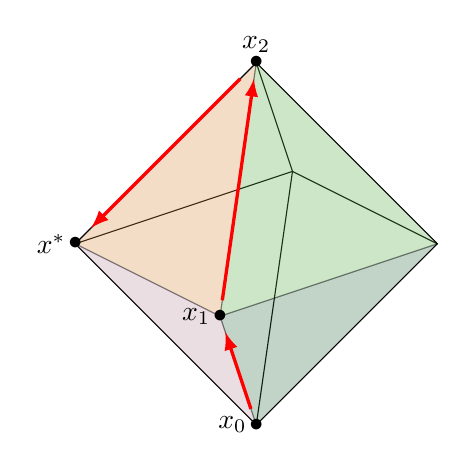
\begin{tikzpicture}[scale=4.6]
  \coordinate (A1) at (0, 0);
  \coordinate (A2) at (0.6, 0.2);
  \coordinate (A3) at (1, 0);
  \coordinate (A4) at (0.4, -0.2);
  \coordinate (B1) at (0.5, 0.5);
  \coordinate (B2) at (0.5, -0.5);
  
  \draw (A1) -- (A2) -- (A3);
  \draw (B1) -- (A2) -- (B2);
  
  \draw[fill=cof, opacity=0.3] (A1) -- (A4) -- (B1);
  \draw[fill=pur, opacity=0.3] (A1) -- (A4) -- (B2);
  \draw[fill=greeo, opacity=0.3] (A3) -- (A4) -- (B1);
  \draw[fill=greet, opacity=0.3] (A3) -- (A4) -- (B2);
  \draw (B1) -- (A1) -- (B2) -- (A3) --cycle;
  \node[draw=none] (a1) at (A1) {$\bullet$} ;
  \draw[left] (A1) node {$x^*$};
  \node[draw=none] (b2) at (B2) {$\bullet$} ;
  \draw[left] (B2) node {$x_0$};
  \node[draw=none] (a4) at (A4) {$\bullet$} ;
  \draw[left] (A4) node {$x_1$};
  \node[draw=none] (b1) at (B1) {$\bullet$} ;
  \draw[above] (B1) node {$x_2$};

  \draw[very thick, -latex, red] (b2) -- (a4) ;
  \draw[very thick, -latex, red] (a4) -- (b1) ;
  \draw[very thick, -latex, red] (b1) -- (a1) ;
\end{tikzpicture}

